\documentclass[a4paper, 12pt]{article}
\usepackage{comment} % enables the use of multi-line comments (\ifx \fi) 
\usepackage{lipsum} %This package just generates Lorem Ipsum filler text. 
\usepackage{graphicx}
\usepackage{wrapfig}
\usepackage{fullpage} % changes the margin
\usepackage{natbib}
\usepackage{url}
\usepackage{float}





\begin{document}
\noindent
\Huge\textbf{Artificial Neural Networks} \\  
\normalsize P.-Y. Lu, Y.-Y. Chang, and S.-K. Hsieh.  Causing emotion in collocation:  An exploratory data analysis. In Proceedings of the 25th Conference on Computational Linguistics and Speech Processing (ROCLING 2013), pages 236---249, 2013.
\\ \\
\begin{center}
	\textbf{Jishnu Dev Roy} \\
\end{center}




\section*{Introduction}
\begin{quote}
"...a computing system made up of a number of simple, highly interconnected processing elements, which process information by their dynamic state response to external inputs.”\end{quote}   - Dr. Robert Hecht-Nielsen,\\ The inventor of the first neurocomputer.\\

Recently the study of the ANN models is gaining importance because of their potential to offer solutions to some of the problems  which  have been intractable by standard serial computers in the areas of computer science and artificial intelligence.   Neural  networks are  better suited for achieving human-like  performance in the fields such as speech processing, image recognition,  machine  vision, robotic control, etc \cite{lee1992short}.

An artificial neural network (ANN) as a  computing system is made up of a  number of simple, and highly  interconnected  processing  elements,  which  processes  information by its dynamic state response to external  inputs.

The architectures of ANNs are motivated by models of biological neural networks which can recognize patterns and learn from their interactions with the environment. The highly sophisticated human brain, which contains more than 100 billion neurons and trillions of interconnections, is able to learn quickly from experience and is generally superior to any existing machine in tasks involving recognition, learning, and control \cite{hsu1995artificial}.





\section*{Theoretical background}

\begin{itemize}

	\item \textbf{ Neurons:}	Neurons (also called nerve cells) or simply neurons are the fundamental units of the brain and nervous system, the cells responsible for receiving sensory input from the external world via dendrites, process it and gives the output through Axons. 

\begin{figure}[H]
	\begin{center}
		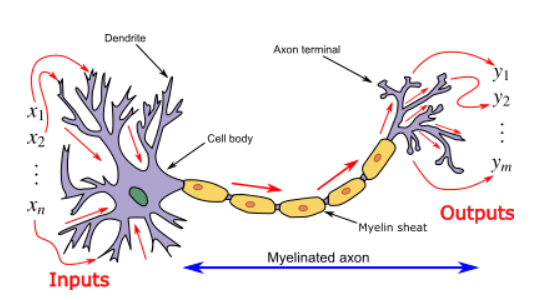
\includegraphics[scale=.8]{images/neuron}
		\caption{Biological Neuron \cite{towardsDataScience} }
		\label{fig:Neuron}
	\end{center}
\end{figure}


\item \textbf{ Perceptron:} A single layer neural network is called a Perceptron. It gives a single output.

\begin{figure}[H]
	\begin{center}
		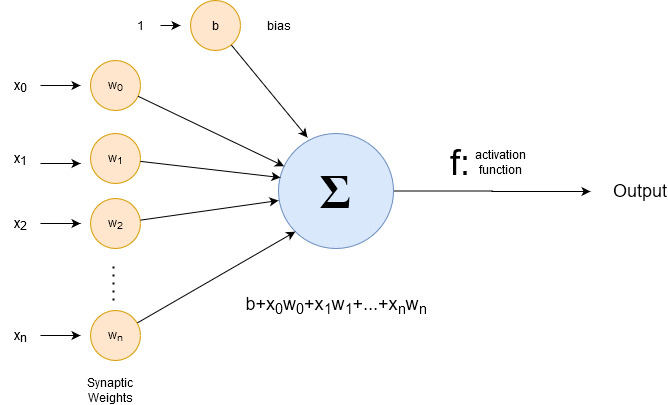
\includegraphics[scale=.6]{images/perceptron}
		\caption{Single Layer Perceptron }
		\label{fig:perceptron}
	\end{center}
\end{figure}
In the above figure, for one single observation, x0, x1, x2, x3...x(n) represents various inputs to the network. Each of these inputs is multiplied by a connection weight. The weights are represented as w0, w1, w2, w3….w(n) . Weight shows the strength of a particular node.
\end{itemize}

\section*{Applications}

\begin{itemize}
	
	\item \textbf{  Image Processing and Character recognition:}	Given ANNs ability to take in a lot of inputs, process them to infer hidden as well as complex, non-linear relationships, ANNs are playing a big role in image and character recognition. Character recognition like handwriting has lot of applications in fraud detection (e.g. bank fraud) and even national security assessments. Image recognition is an ever-growing field with widespread applications from facial recognition in social media, cancer detention in medicine to satellite imagery processing for agricultural and defense usage. The research on ANN now has paved the way for deep neural networks that forms the basis of “deep learning” and which has now opened up all the exciting and transformational innovations in computer vision, speech recognition, natural language processing — famous examples being self-driving cars.
	
	\item \textbf{ Forecasting:}	Forecasting is required extensively in everyday business decisions (e.g. sales, financial allocation between products, capacity utilization), in economic and monetary policy, in finance and stock market. More often, forecasting problems are complex, for example, predicting stock prices is a complex problem with a lot of underlying factors (some known, some unseen). Traditional forecasting models throw up limitations in terms of taking into account these complex, non-linear relationships. ANNs, applied in the right way, can provide robust alternative, given its ability to model and extract unseen features and relationships. Also, unlike these traditional models, ANN doesn’t impose any restriction on input and residual distributions.
	
	\item \textbf{ Financial:}	  Real estate appraisal, loan advisor, mortgage screening, corporate bond rating, portfolio trading program, corporate financial analysis, currency value prediction, document readers, credit application evaluators.
	\item \textbf{ Industrial:}	  Manufacturing process control, product design and analysis, quality inspection systems, welding quality analysis, paper quality prediction, chemical product design analysis, dynamic modeling of chemical process systems, machine maintenance analysis, project bidding, planning, and management.
	\item \textbf{ Anomaly Detection:}	  As ANNs are expert at recognizing patterns, they can also be trained to generate an output when something unusual occurs that misfits the pattern.
	\item \textbf{ Medical:}  Cancer cell analysis, EEG and ECG analysis, prosthetic design, transplant time optimizer.
	\item \textbf{ Aerospace:}	Autopilot aircrafts, aircraft fault detection.
	
\end{itemize}




			
			





\section*{Conclusion}
The ANN is the very useful model and the ANN could be applied in problem-solving and machine learning. The computing World has a lot to gain from the Neural Network. Thus, Their ability to learn by example makes them very flexible and powerful. Hence to best utilize the ANN for different problems, it is essential to understand the potential as well as the limitations of the Neural Network.


%=============================================
\bibliographystyle{plain}
\bibliography{Cites.bib}

\end{document}


\ifx
Comments!
\fi

% ===========

\ifx

%==============

% References if you want it manual

% \bibitem{Robotics} Fred G. Martin \emph{Robotics Explorations: A Hands-On Introduction to Engineering}. New Jersey: Prentice Hall.

% \bibitem{Flueck}  Flueck, Alexander J. 2005. \emph{ECE 100}[online]. Chicago: Illinois Institute of Technology, Electrical and Computer Engineering Department, 2005 [cited 30
% August 2005]. Available from World Wide Web: (http://www.ece.iit.edu/~flueck/ece100).

